\documentclass{article}
\usepackage{times}
\usepackage[titletoc]{appendix}
\usepackage{graphicx}
\usepackage{lineno}
\usepackage{multirow}
\usepackage[english]{babel}
\usepackage{typearea} 
\usepackage{amssymb}
\usepackage{amsfonts}
\usepackage{amsmath}
\usepackage{enumerate}
\usepackage{mathtools}
\usepackage{graphicx}
\usepackage{wrapfig}
\usepackage{lscape}
\usepackage{rotating}
\newcommand{\Fig}[1]{Figure~\ref{fig:#1}}

\renewcommand{\baselinestretch}{1.5}
\newcommand{\bbar}[1]{\overline{#1}}

\newcommand\scalemath[2]{\scalebox{#1}{\mbox{\ensuremath{\displaystyle #2}}}}
\renewcommand{\familydefault}{\sfdefault}

\usepackage[font={small},labelfont={bf},justification=justified,margin=0.5cm]{caption}

\renewcommand{\thesection}{}
\renewcommand{\thesubsection}{\arabic{section}.\arabic{subsection}}

\usepackage{color}
	 \definecolor{darkred}{rgb}{0.75,0,0}
%	 \definecolor{darkgreen}{rgb}{0,0.5,0}
	 \definecolor{darkblue}{rgb}{0,0,0.75}
%	 \definecolor{magenta}{rgb}{0,0,0.75}
\newcommand{\cha}[1]{\textcolor{darkgreen}{(#1)}}
\newcommand{\maria}[1]{\textcolor{darkred}{(#1)}}


\usepackage{hyperref}
\definecolor{darkgreen}{rgb}{0.1,0.6,0.3}
\definecolor{darkred}{rgb}{0.6,0.3,0.1}
\hypersetup{
    colorlinks=true,       % false: boxed links; true: colored links
    linkcolor=blue,          % color of internal links (change box color with linkbordercolor)
    citecolor=darkgreen,        % color of links to bibliography
    filecolor=magenta,      % color of file links
    urlcolor= black           % color of external links
}

\title{\vspace*{-22mm}\bf Assessing integrated management practices for control of \textit{Sclerotinia sclerotiorum} in oilseed rape}


\date{}

\begin{document}
\linenumbers
\maketitle

%\begin{abstract}
%Here, we investigate how the combination of these strategies affects the build-up of the fungi reservoir in the soil and the seasonal yield gain. We use a theoretical model that imitates the infection dynamics for oilseed rape within and between harvesting seasons. For each season, the soil reservoir -- here, spore bank -- and yield are approximated depending on the infected plant area. The results show that integration of multiple strategies makes short rotations successful in preventing an infection build-up and provide long-term control of the epidemic. 





\section{Introduction}
Every year, plant diseases affect crops, diminishing the farmers' yields. Sclerotinia stem rot (SSR) is a disease caused by the fungi \textit{Sclerotinia sclerotiorum} which affects several commercial crops causing white mould and stem rot. Here we focus on how it affects oilseed rape (OSR), \textit{Brassica napus}, where infection can cause yield losses of up to 60\% \cite{twengstrom:CropP:1998, rothmann:SAJC:2018}. The epidemic can be reduced by using crop rotations or foliar fungicides, but farmers rarely achieve total control using a single method. Integrated pest management (IPM) is regarded as a potential solution \cite{derbyshire:PP:2016}. IPM, by definition, takes genetic, chemical and biological control as complementary, and uses all suitable techniques to maintain the population levels of a pathogen below those causing economic losses \cite{Smith and Reynold 1966: Dent 1991, kogen:1998:ARE}. The use of IPM in \textit{Sclerotinia} could improve current practices by combining both crop rotations and fungicides, and adding alternative strategies such as crop variants with partial genetic resistance or biocontrol \cite{derbyshire:PP:2016}. 
\\

\textit{Sclerotinia sclerotiorum} is a soil-borne fungus which proliferates in moist conditions and has a monocyclic life cycle, i.e. it relies on a primary inoculum to develop, without producing secondary inocula. To survive, it forms a structure called sclerotia which allows it to remain in the soil across seasons. When the sclerotium germinates, it produces fruiting bodies which release ascospores to infect the host. In OSR, the ascospores infect the petals in the flowering season, which fall and cause damage to the stem. In the infected stems, more sclerotia are produced, reaching the soil and closing the life cycle \cite{derbyshire:PP:2016, heffer:TPHI:2007}. The severity of the disease depends very much on weather conditions -- it is favoured by high humidity and warm temperatures --, but farming practices are also considered when assessing the risk, mainly the OSR cropping frequency in the field \cite{koch:PhytoP:2007}. 
\\

A common cultural practice that prevents SSR is the rotation with cereals such as wheat or barley. Because these cereals are non-hosts for the pathogen, the soil sclerotia remnants cannot reproduce \cite{}. However, sclerotia can remain viable in the soil for up to 8-10 years \cite{adams:PhytoP:1979}: this requires farmers to apply long rotations with multiple years of break crops. Otherwise, in short rotations, the infection can build up from season to season due to the accumulation of sclerotia: this phenomenon has accentuated in the last decade as the frequency of OSR in rotations has increased from more than four break seasons to 1-year break \cite{OSR:HGCA:2014}. The use of fungicides offers another viable control method.  The application of fungicides in the early flowering time as prophylaxis can prevent the infection. However, if the ascospores have reached the petals before the spraying or the risk of infection is very low, the fungicides have limited effect and so this results in economic losses \cite{}.There are no known cultivars with full resistance to SSR, but varieties with partial resistance or some disease tolerance have been identified \cite{}. 
\\

Here, we study IPM strategies to control SSR of OSR by adapting a  generic model of seasonal rotations of host and non-host crops \cite{bargues-ribera:PCB:2019}. Taking the implementation of seasonal rotations, we expand the model to include both the fungicide effect and partial resistant crop variants. We aim to study how the integration of two or three control strategies -- rotations, fungicides and genetic resistance -- can improve the management of OSR. For that, we simulate host infection dynamics within and between seasons. The season output is coupled to two variables of interest: yield gain and spore bank, i.e. changes of sclerotia quantities in the soil. Overall, the model informs that combined strategies can succeed in controlling the infection using short rotations, even if the fungicide efficiency and the level of genetic resistance are low. 

\section{Methods}


\subsection{Model description}


The model is based on \cite{bargues-ribera:PCB:2019}, which focuses on crop rotations in a single field. In each season, one crop type is cultivated: a host crop promotes the infection, while a non-host crop prevents it. Plant-pathogen dynamics are modelled within and across harvesting seasons. The model uses hybrid time: within a season, the disease follows infection spread in continuous time; between seasons, time is discrete and population densities are updated. The infection is coupled to the calculation of seasonal yield. 

In the model presented here, the host crop is oilseed rape (OSR). Disease control can be achieved by rotations with break crops (non-host) as a form of cultural control (C); but In contrast to \cite{bargues-ribera:PCB:2019}, we extend management strategies to the use of genetic resistance (G) and the application of fungicides (F). Infection is modelled from the first season. In each season, we model healthy and infected crop densities. After each season, two discrete variables are updated according to the status of the infection: spore bank (equivalent to the number of soil sclerotia) and yield. We explore infection dynamics in rotation sequences of 20 seasons of length, and we assess the total OSR yield and infection build-up based on the final spore bank. Results are compared for the cultivation of consecutive OSR (null case) and the use of one, two or three control strategies (C, G, F) (Fig. \ref{fig:cube}). 

\subsection{Within and between season infection}

The infection is modelled using a system of two coupled differential equations which indicate the dynamics of the healthy and the infected crop density. Initially, there is a total crop density of 100 plants/m\textsuperscript{2}, considering both healthy and infected densities ($h(t=0) + i(t=0) = 100$). Healthy plants do not reproduce, their density decreases when they get infected at rate $\beta$ (Eq. 1). The primary inoculum ($i_0$) determines the initial value of the infected crop density ($i(t=0)$), which value increases during the season. This increase depends on the rate of infection $\beta$, the available healthy crop density $h(t)$, the current infected density $i(t)$ and the influx of primary inoculum $i_0$ (Eq. 2). The infected plants die at a rate of $\delta$. 

At the end of the season, we calculate the area under disease progress curve AUDPC ($A$), which indicates disease intensity over time. To do so, we approximate the area under the curve (i.e. the definite integral) of the infected plant density. We use the trapezoidal method \cite{madden:2007} using the beginning and the end of the season as time interval (Eq. 7). With the AUDPC we update the spore bank $S(t)$, which conserves a proportion $\eta$ from the last season and adds sclerotia during the infection of the current season $\gamma A$ (Eq. 4). The yield for each season ($Y(t)$) depends on the crop infection status at the moment of the harvest, i.e. the final value of $i(t)$ (Eq. 5). The primary inoculum for the next season is set according to the spore bank using $\epsilon$. If fungicides are applied, the primary inoculum is reduced by 1 - $\mu$, where $\mu$ is the fungicide efficiency (Eq. 6). The spore bank builds up when there are consecutive seasons of the susceptible crop. If a break crop is grown then there is no build up in the spore bank and so the infection potential is reduced. With a resistant crop, the pathogen fitness $w$ is reduced depending on $\rho$, which lowers the rate of infection spread and so the increase in spore bank is smaller. 
%\begin{equation} 
%
%\end{equation}

\begin{eqnarray}
\dot{h} &=& - w \beta h (i + i_0) \\
\dot{i} &=& w \beta h (i + i_0) - \delta i \\
w & = & 1 - \rho \\
S (t) &=& \eta S(t-1) + \gamma A(t) \\
Y (t) &=& Y_{max} - \alpha i (t) \\
i_0 &=& (1 - \mu) \epsilon S(t) \\
A(t) &=& \frac{i(t-1) + i(t)}{2} \Delta t
\end{eqnarray}

\subsection{Characterisation of cropping strategies}

The dynamics within one season depend on the initial inoculum $i_0$ and the rate of infection spread $\beta$; which lead to an end-of-season stem rot severity $i(t)$. The initial inoculum calculates on the amount of spore bank $S(t)$, and it changes with the application of fungicides, with fungicide efficiency $\mu$. The rate of infection spread varies with the crop type: when the crop has some resistance, pathogen fitness is decreased ($w < 1$). 
%Besides, the crop type also modifies the seasonal yield: a resistant cultivar may provide a different number of plants, pods or seeds than a standard susceptible cultivar. 
The four management interventions that are explored are: 

\begin{itemize}
\item No control (null strategy, $\varnothing$). We grow consecutive seasons of a susceptible variety of oilseed rape (all OSR). Because the crop is susceptible, the pathogen has full fitness for the host crop ($w = 1$). Fungicides are not applied ($\mu = 0$). 

\item Cultural control (single strategy, C). We alternate oilseed rape and break crops in seasonal rotations (repetition of OSR-BC). In seasons of OSR, the pathogen has full fitness for the host crop ($w = 1$). In seasons of break crop, the primary inoculum is null ($i_0 = 0$). Fungicides are not applied ($\mu = 0$). 

\item Fungicide control (single strategy, F). We cultivate consecutive seasons of oilseed rape (all OSR). Because the crop is susceptible, the pathogen has full fitness for the host crop ($w = 1$). Fungicides are applied ($\mu > 0$), reducing the primary inoculum. 

\item Genetic control (single strategy, G). We grow consecutive seasons of oilseed rape (all OSR). However, the pathogen is assumed to have a reduced ability to infect this crop compared to the susceptible. This is simulated by reducing the pathogen fitness for the host crop ($w < 1$). Fungicides are not applied ($\mu = 0$). 
\end{itemize}

When the control strategies are applied together, the specifications of each strategy are combined, as shown in Table \ref{table:charac}.


\begin{table}[h]
\caption{\label{table:c}\textbf{List of strategies and their characterisation}}
\begin{tabular}{llll}%{|ll|l|l|}

	\multicolumn{4}{c}{}\\
	\hline
	Strategy & Seasonal pattern & Pathogen fitness & Fungicide efficiency \\
	\hline
	$\varnothing$ & OSR & $w = 1$ & $\mu = 0$ \\
	C & OSR-BC & $w = 1$ & $\mu = 0$ \\
	G & OSR & $w < 1$ & $\mu = 0$ \\
	F & OSR & $w = 1$ & $\mu > 0$ \\
	CG & OSR-BC & $w < 1$ & $\mu = 0$ \\
	CF & OSR-BC & $w = 1$ & $\mu > 0$ \\
	GF & OSR & $w < 1$ & $\mu > 0$ \\
	CGF & OSR-BC & $w < 1$ & $\mu > 0$ \\
	\hline
\end{tabular}
\end{table}

\begin{figure}
\caption{\label{fig:cube}\textbf{Space of possible control strategies.} Starting from the null strategy ($\varnothing$), we can apply either cultural (C), fungicide (F) or genetic (G) control. From these points, we can add a second strategy and use cultural-fungicide (CF), cultural-genetic (CG) or fungicide-genetic (FG) double control methods. Finally, we can combine the three strategies and use cultural-fungicide-genetic control (CFG). }
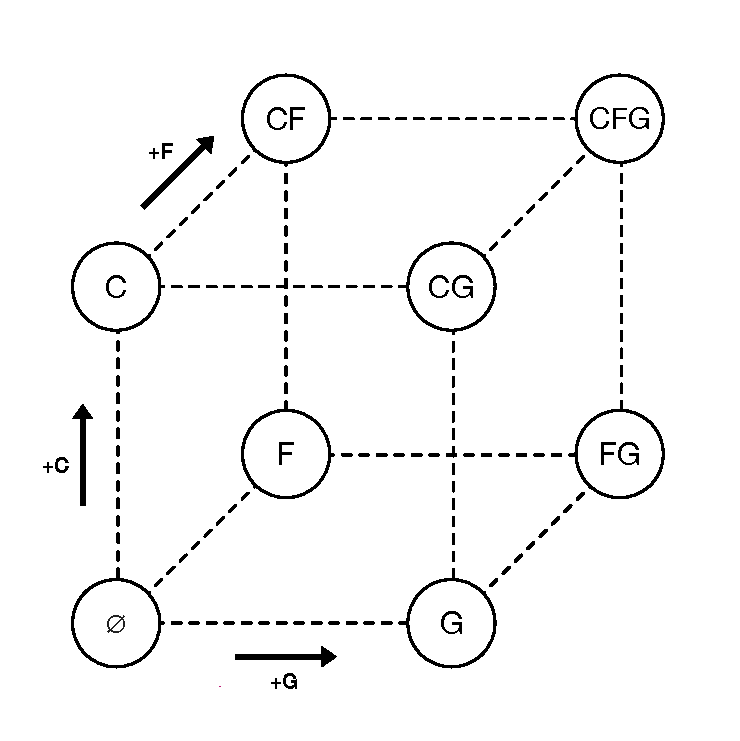
\includegraphics[width=0.5\columnwidth]{SCL_Fig/SCL_Fig1.pdf}
\end{figure}


\subsection{Parametrisation}


%\subsection{Parametrisation}
%
\begin{table}[h]
\caption{\label{table:params}\textbf{List of parameter values, with description and feasible range.}}
\begin{tabular}{llll}%{|ll|l|l|}

	\multicolumn{4}{c}{}\\
	\hline
	Parameter & Value & Description & Range \\
	\hline
	$\alpha$ & 0.035 &Yield loss due to infection& 0 - 0.05\\
	$\beta$ & 0.04&Rate of infection& 0 - 1\\
	$\gamma$ & 1&Seasonal spore gain& 0 - 1\\
	$\delta$ &  0.3&Death rate of infected plants& 0 - 1\\
	$\epsilon$ & 0.15&Seasonal inoculum& 0 - 1\\
	$\eta$ & 0.6&Seasonal spore survival& 0 - 1\\
	$\mu$ & variable &Fungicide efficiency& 0 - 1\\
	$\rho$ & variable &Genetic resistance& 0 - 1\\
	\hline
\end{tabular}
\end{table}

The equations have several parameters (Table \ref{table:params}) which values define the infection dynamics. In consequence, their optimisation can approximate the results observed in crop fields. Here we describe the relationship of these parameters with descriptive variables found in field reports or previous literature. We show an example table (Table \ref{table:data}) from \cite{gladders:HGCA:2008}, which shows values for stem rot index and yield for untreated and treated fields of winter OSR in the years 2006 and 2007, when there was a severe epidemic of SSR in the UK. From all values, we have selected the fields Hereford 1 and 3, the year 2007, as their cultivar varieties (Catalina and Castille, respectively) showed both severe stem rot and a significant response to fungicide treatment. We can use it as a guide for parametrisation, as explained: 

\begin{itemize}
\item Within a season, the rate of infection $\beta$ determines the infected plant density at the end of the season $i$. In reports, we can relate $i$ to the stem rot index. The stem rot index determines the percentage of infected plants, and it is used as indication of disease severity. In the data, the average stem rot index, without treatment, is 60.5\% (s = 10.6). In our simulation, if starting with an initial spore bank of $S(t = 0) = 50$, which could relate to severe infection; $i(t = 1) = 66.36$, which compared to the total plant density ($i(t=1) + h(t = 1) = 89.67$), is $74\%$ of infected plants. Thus, infection is overestimated according to the assumed initial inoculum. These results also depend on the death rate of infected plants $\delta$, for which we do not have any data. 

\item Within season dynamics also determine the yield. In the report, the infected fields yielded on average 2.6 t/ha. The maximum yield with treatment was 4.7 t/ha. This can be indicative of an approximated maximum yield of 5 t/ha without infection. An $Y_{max}$ = 5t/ha is realistic for winter oilseed rape cultivars with high yield \cite{} and corresponds to an approx 50\% yield loss in the data for severe infection. When calculating yield under infection, we use a function of the infected area: the yield depends on the plant seeds, which are reduced or damaged when the plant dies or the infection is severe; with yield loss not exceeding 50-60 \%. In our simulations, for values in \ref{table:params} and initial spore bank of $S(t = 0) = 50$, we obtain a yield of 2.7 t/ha, close to the average.

\item Between seasons, a proportion of the spore bank remains in the soil, as sclerotia can survive up to 8-10 years. The parameter $\eta$ regulates the decay of soil sclerotia. In our simulations, the spore bank after 5 seasons of break crop (null increase) is reduced to less than 10 \% of the initial value, and after 10 seasons of break crop, less than 1\% of the initial spore bank remains.   


\item Regarding fungicide application, the table compares stem rot index in untreated and treated fields, which can approximate the efficiency of the fungicide. However, in our study we focus on the exploration of the fungicide efficiency parameter $\mu$, as the resulting control can depend on the fungicide type and dosage.
\end{itemize}

The parameter values can be fit to the field report or other sets of data, using optimisation algorithms that adjust them to obtain the expected results. The current values aim to be useful to test the model and explore general outcomes of the integration of strategies. 


\begin{table}[h]
\caption{\label{table:data}\textbf{Data from Gladders et al., 2008}}
\begin{tabular}{cccp{20mm}p{20mm}p{20mm}p{20mm}} %.    .   {llll|||}%{|ll|l|l|}
	\multicolumn{7}{c}{}\\
	\hline
	Site & Year & Cultivar & Stem rot \newline index\newline (untreated) & Stem rot \newline index \newline (treated) & Untreated yield & Treated yield (untreated + response)\\
	\hline
	Hereford 1 & 2007 & Catalina & 57.3 & 9.6 & 3.0 & 4.7 \\
	Hereford 3 & 2007 & Castille & 72.3 & 13.0 & 2.6 & 3.4 \\
	Hereford 1 & 2007 &Catalina & 67.7 & 11.7 & 2.4 & 4.5 \\
	Hereford 3& 2007& Castille & 44.8 & 8.4 & 2.4 & 3.3 \\
	\hline
	 &  & Average & 60.5 \newline (s = 10.6) & 10.7 \newline (s = 1.8) & 2.6 \newline (s = 0.2) & 4.0 \newline (s = 0.6) \\
	 \hline
	 &  & Defined range & 0-100 & 0-100 & 0-5 & 0-5 \\
	\hline
\end{tabular}
\end{table}


%
%To parametrise the model, we have started with a single season of the null strategy, where susceptible OSR is cultivated. To determine a realistic curve of infection, we have taken values from \cite{gladders:HGCA:2008}. The report shows values for stem rot index and yield for untreated and treated fields of winter OSR in the years 2006 and 2007, when there was a severe epidemic of SSR in the UK. The stem rot index relates to the percentage of host tissues damaged by the disease, which in our model is represented by $i(t)$. From all values, we have selected the fields Hereford 1 and 3, the year 2007, as their cultivar varieties (Catalina and Castille, respectively) showed severe stem rot and a significant response to fungicide treatment (Lioness cultivar also showed significant treatment response in some fields, but not severe infection). To compare yields, we have defined a maximum yield of $Y_{max} = 5$ (in tonnes per hectare, t/ha), which would be realistic for high-yield winter OSR and relates to both (a) the maximum yield value observed in this data ($ Y = 4.74$), and (b) the minimum yield ($ Y = 2.41$) in severe infection which should correspond to 40-50\% of the maximum (due to expected 50-60\% of yield loss \cite{}). Table \ref{table:data} shows the values of interest from the data. 
%\\
%
%\begin{table}
%\caption{\label{table:data}\textbf{Data from report X}}
%\begin{tabular}{cccp{20mm}p{20mm}p{20mm}p{20mm}} %.    .   {llll|||}%{|ll|l|l|}
%	\multicolumn{7}{c}{}\\
%	\hline
%	Site & Year & Cultivar & Stem rot \newline index\newline (untreated) & Stem rot \newline index \newline (treated) & Untreated yield & Treated yield (untreated + response)\\
%	\hline
%	Hereford 1 & 2007 & Catalina & 57.3 & 9.6 & 3.0 & 4.7 \\
%	Hereford 3 & 2007 & Castille & 72.3 & 13.0 & 2.6 & 3.4 \\
%	Hereford 1 & 2007 &Catalina & 67.7 & 11.7 & 2.4 & 4.5 \\
%	Hereford 3& 2007& Castille & 44.8 & 8.4 & 2.4 & 3.3 \\
%	\hline
%	 &  & Average & 60.5 \newline (s = 10.6) & 10.7 \newline (s = 1.8) & 2.6 \newline (s = 0.2) & 4.0 \newline (s = 0.6) \\
%	 \hline
%	 &  & Defined range & 0-100 & 0-100 & 0-5 & 0-5 \\
%	\hline
%\end{tabular}
%\end{table}
%
%Taking into account the average values and their standard deviation, we have adjusted the spread rate ($\beta = 0.04$) and the intrinsic death rate ($\delta = 0.3$) to have fitting curves. Yield value is reduced proportionally to the pathogen depending on $\alpha$ ($\alpha = 0.035$) (Fig. \ref{fig:parwithin}).
%When setting the fungicide effect, with very high efficiency ($\mu = 0.95$) results are comparable to the data (Fig. \ref{fig:par_within}). However, the fungicide type and dose can vary the effect \cite{}. Besides, we cannot use this data to determine the resistance level of the genetic control strategy. In consequence, we explore the control provided by different values of fungicide efficiency and genetic resistance (see next section).
%
%\begin{figure}
%\includegraphics[width=\columnwidth]{SCL_Fig2.pdf}
%\caption{\label{fig:parwithin}\textbf{Stem rot and yield values after a single season of OSR, with and without fungicides.} In all panels, we plot the simulation results after one season of OSR ($\beta = 0.04$ and $\delta = 0.3$), starting from different values of initial spore bank (range 0 to 100, units of 1). We indicate the percentage of infected crop area (left panels), and the percentage of yield obtained (right panels) at the end of the season. Horizontal span (magenta) indicates the mean value (line) and standard deviation (shadow) in the reported sample. Vertical line (dashed, black) indicates an initial spore bank of $S = 50$, as a reference to characterise severe infection. In the top panels, no fungicides are applied ($\mu = 0$), while in the bottom panels, fungicides are applied ($\mu = 0.95$).}
%\end{figure}
%
%Apart from the within-season dynamics of infection, we also characterise the between-season dynamics. In the field, consecutive seasons of OSR can provoke an infection build-up from season to season due to the accumulation of sclerotia in the soil. The model \cite{vosough:ACAE:2013} estimated the build-up rate of sclerotia in the soil and the associated yield losses in five consecutive years of OSR cultivation. Both the build-up and the yield loss follow a sigmoid curve. We have adjusted the parameters defining the change in spore bank and initial inoculum ($\eta = 0.6$, $\gamma = 1$,$\epsilon = 0.15$) to imitate qualitatively the build-up in the previous model. We have started with a minimal spore bank ($S(t = 0) = 1$), from which the build-up range is broader (Fig. \ref{fig:parbetween}). To note, their expected yield loss for the fifth season is 76\%, which we consider too high compared to other reports which indicate a maximum yield loss of 50-60\% \cite{} and this affects the fitting of the curve.
%
%\begin{figure}
%\includegraphics[width=\columnwidth]{SCL_Fig3.pdf}
%\caption{\label{fig:parbetween}\textbf{Build-up of sclerotia in soil during 5 seasons of OSR and its corresponding yield loss.} 
%In the left panel, we plot the simulation results for the build-up of the sclerotia in soil, relative to the spore bank value at the end of the 5th season (considered 100\%). The simulated build-up curve (black) corresponds to a starting spore bank of $S = 1$. We compare it to the estimated build-up in \cite{vosough:ACAE:2013} (magenta). In the right panel, we plot the corresponding percentage of yield loss, for our simulation (black) and the previous model estimation (magenta).
%}
%\end{figure}
%
%On the other hand, the proportion of sclerotia remaining in the soil from season to season also affects the performance of break crop seasons. With the indicated value ($\eta = 0.6$), the decay curve of sclerotia in the soil with consecutive break crop seasons fits the expectations that sclerotia can remain in the soil for 8-10 years \cite{} (Fig. \ref{fig:parbreak}).  
%
%\begin{figure}
%\includegraphics[width=0.75\columnwidth]{SCL_Fig4.pdf}
%\caption{\label{fig:parbreak}\textbf{Spore bank decay in consecutive seasons of break crop.} We plot the percentage of spore bank which remains at the end of the number of consecutive break crop seasons indicated in the $x$ axis (solid line). The decay rate is the same for all initial spore bank values. We indicate the intersection with a 50\% reduction of the spore bank (dashed lines).}
%\end{figure}
% 
\section{Results}

The results show the performance for null ($\varnothing$), single (C,F,G), double (CF, CG, FG) and triple (CFG) strategies during 20 seasons, in terms of yield gain and build-up of sclerotia in soil. These results are constrained to an infection which develops from an initial spore bank of $S(t=0) = 10$, unless specified.  Also, we do not consider pathogen evolution, i.e. we assume durable effectiveness of genetic resistance and fungicide application.
 
 
 \subsection{Null strategy ($\varnothing$) and cultural control strategy (C)}
 
\textbf{Null strategy ($\varnothing$)}. We simulate 20 consecutive seasons of OSR. At the end of the 20th season, the values for infected host density and spore bank are maximum in respect to other seasons ($i(t = 20) = 73.76$ plants/m\textsuperscript{2}, $S(t = 20) = 113.36$ a.u.)  (Fig. \ref{figA}). The infection dynamics show a rapid build-up of soil sclerotia in the initial seasons: considering the final spore bank as 100\% of build-up, spore bank at the end of the 6th season reaches more than 80\% of build-up ($S(t = 6) = 94.77$ a.u.). The yield obtained per season decays with time, and at the end of the 20th season we get 48.40\% of the maximum yield ($Y(t = 20) = 2.42$ t/ha). When comparing with the cumulative maximum yield of OSR -- i.e. total yield collected after 20 seasons with 5 t/ha each --, we get 51.12 \% of the total. 
\\
 
 \textbf{Single strategy: cultural control (C)}. We simulate 20 seasons of the rotation OSR-BC (i.e. seasonal alternations of OSR with a break crop BC).  We establish the rotation with a single season of break crop (short rotation) as the default cultural strategy, but we explore how the results change when we increase the number of break crops (long rotation)  (Fig. \ref{figA}). The infection dynamics show that short rotations (OSR-BC) do not prevent a build-up of the infection: the spore bank after the 20th season is increased respect to the initial one ($S(t = 20) = 29.02$ a.u., $S(t = 20) > S(t=0)$). However, longer rotations with three seasons of break crop (OSR-BC-BC-BC) do control the infection and reduce the sclerotia in soil ($S(t = 20) = 1.19$ a.u., $S(t = 20) < S(t=0)$). The maximum infected host density occurs at the last season of OSR for short rotations ($i(t = 20) = 57.73$ plants/m\textsuperscript{2}) and the first season of OSR for 3-break crop rotations ($i(t = 1) = 35.83$ plants/m\textsuperscript{2}). 
 
 When applying cultural control, the cumulative maximum yield of OSR corresponds to the total yield collected during the OSR seasons: 10 seasons in the case of short rotations, 5 seasons for long rotations with 3 break crops. Taking this into account, we get 63.32\% of the total yield for short rotations and 86.48\% of the total yield for long rotations with 3 break crops. 
 
We also explore how different number of break crop seasons after a single season of oilseed rape change the spore bank value  (Fig. \ref{figB}). Results show that the number of break crop seasons needed to control the infection -- i.e. prevent a build-up of sclerotia in the soil -- depends on the initial spore bank value. At low values of spore bank ($S(t = 0) \lesssim 10$), a minimum of 3 break crops are needed to control the infection. However, at high values of spore bank ($S(t = 0) \gtrsim 30$), 1-year of break crop already prevents an infection build-up. 
 
 Because of farmers' interest in increasing the cropping frequency of OSR, we constraint the study of cultural control strategy in combination with genetic control and/or fungicides (CG, CF, CGF) to the application of a single season of break crop.
 
 \begin{figure}
 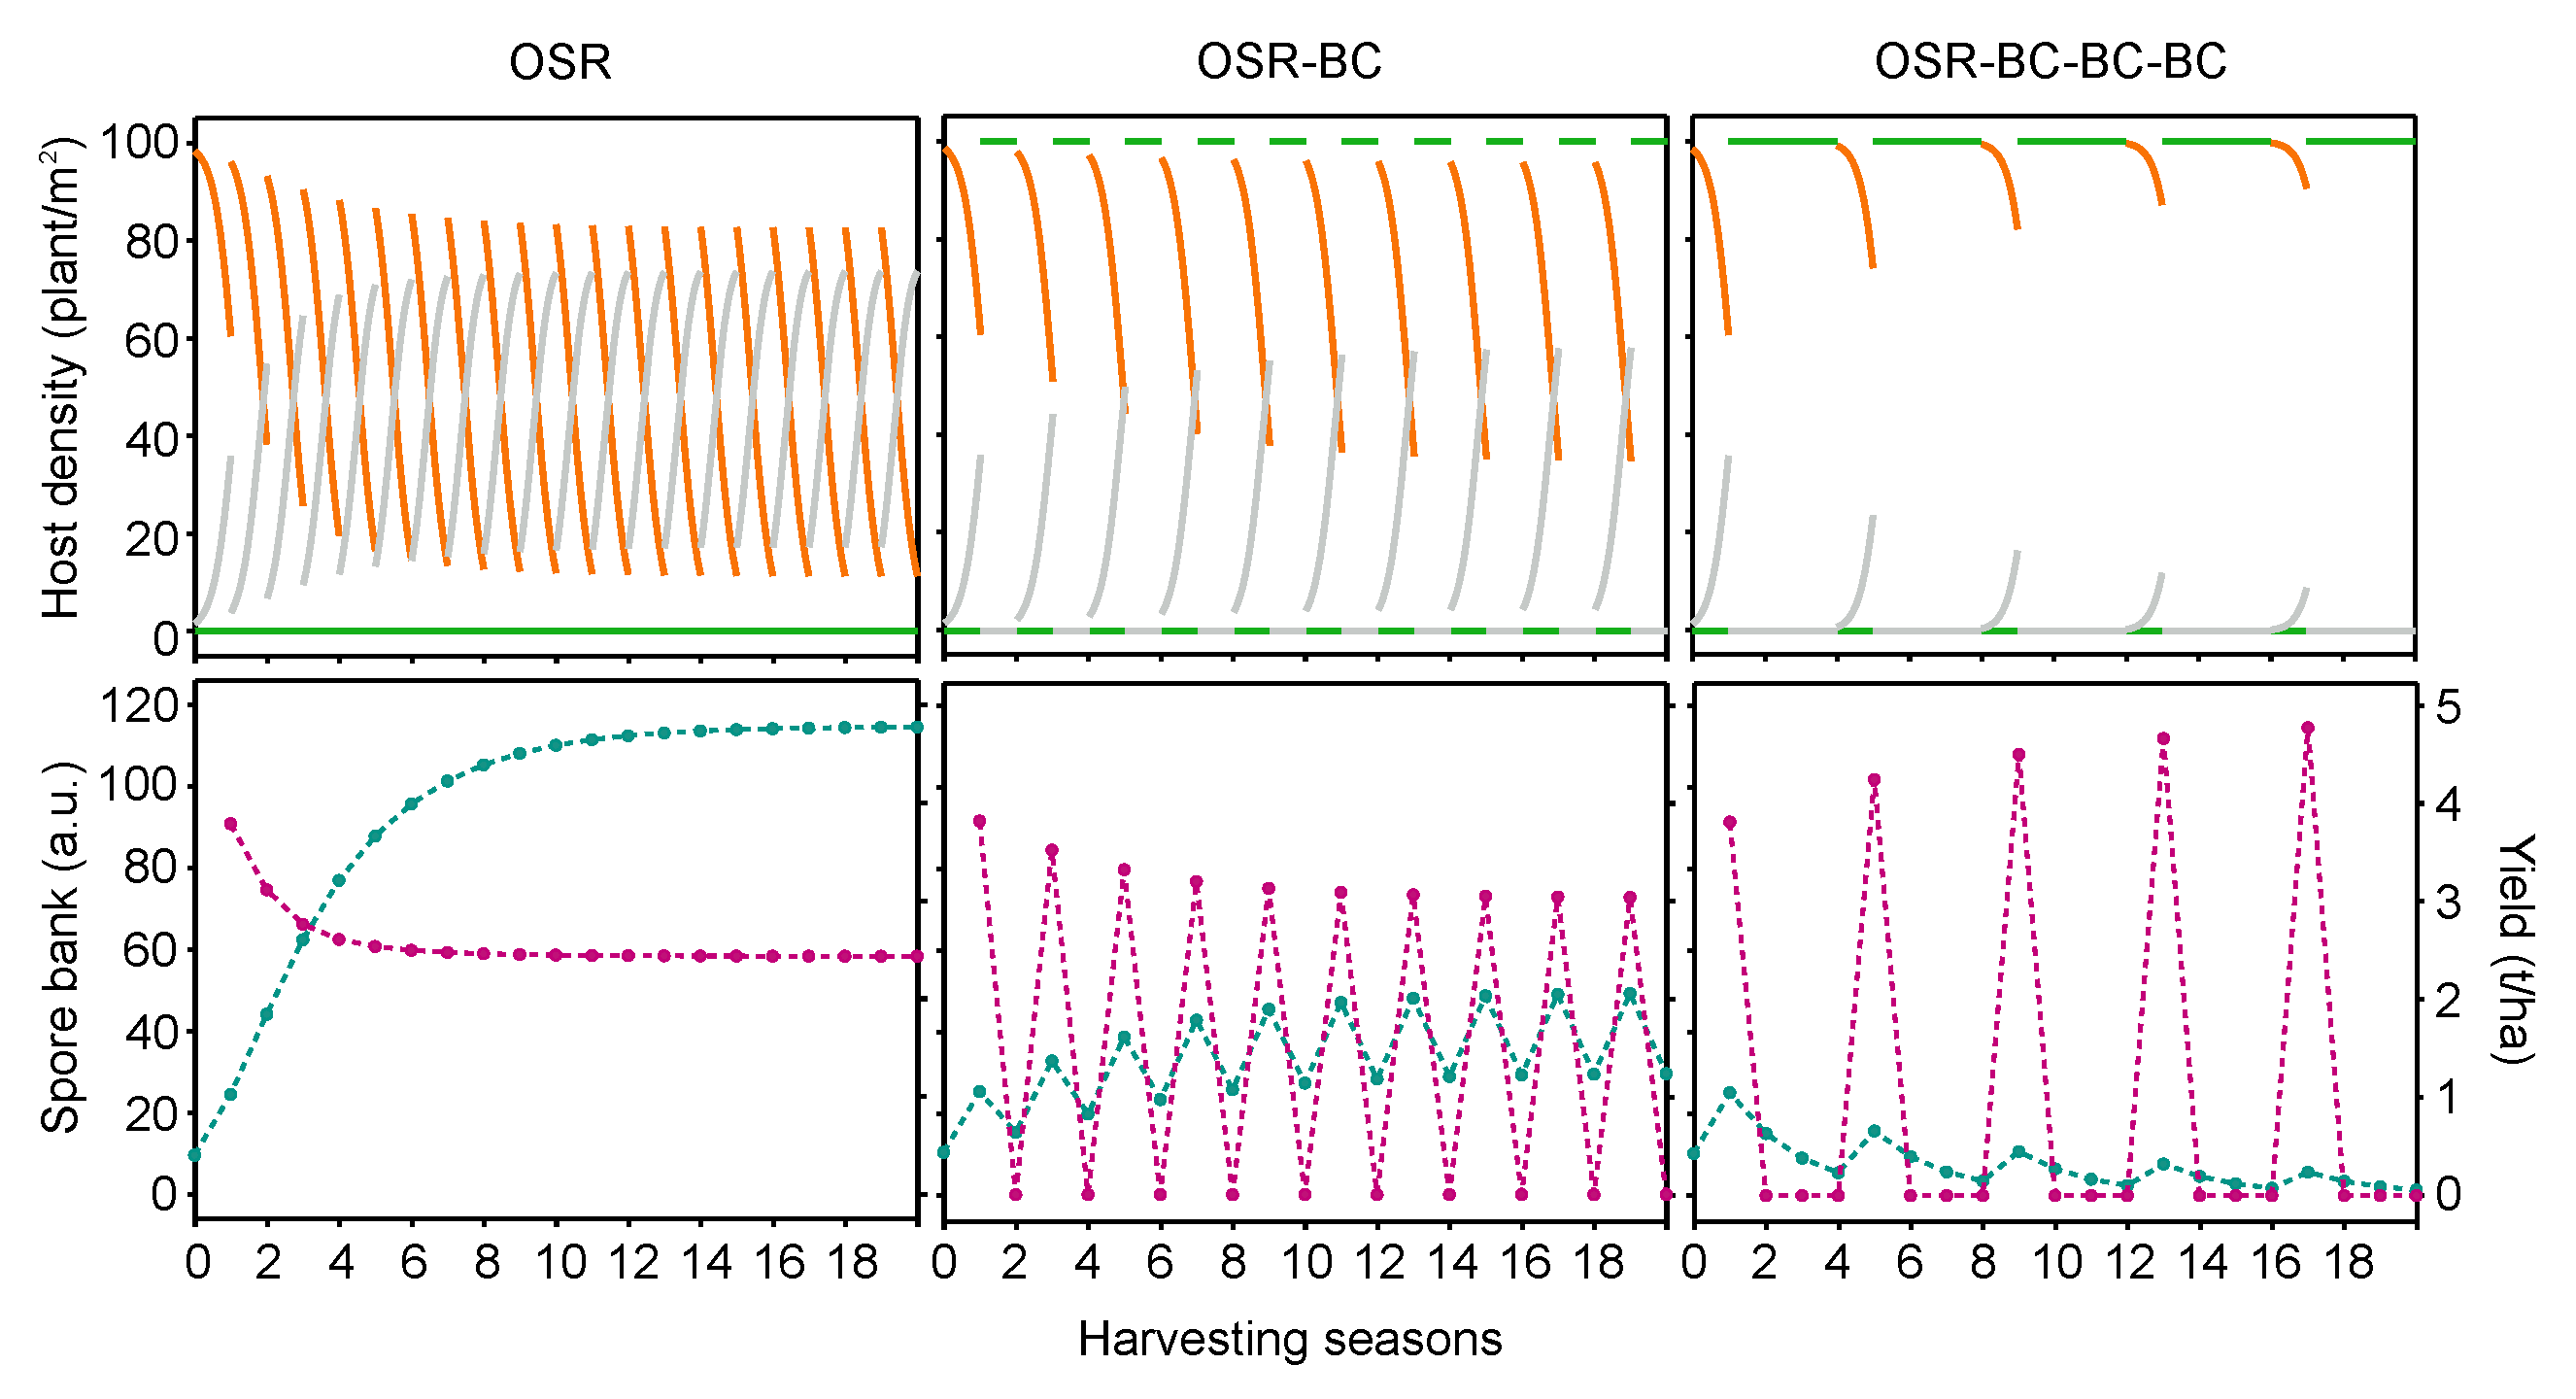
\includegraphics[width=\columnwidth]{SCL_Fig/SCL_FigA.pdf}
\caption{\label{fig:figA}\textbf{Infection dynamics, with spore bank and yield seasonal updates, for the null ($\varnothing$) and cultural control (C) strategies, during 20 harvesting seasons.} Top panels indicate infection dynamics, which show variations in healthy crop area (orange for oilseed rape, green for break crop) and infected crop area (grey). Dynamics are continuous within the season and discrete between the seasons. Bottom panels show the discrete update of spore bank (turquoise) and yield (magenta) variables after each season. }
\end{figure}
 
  \begin{figure}
 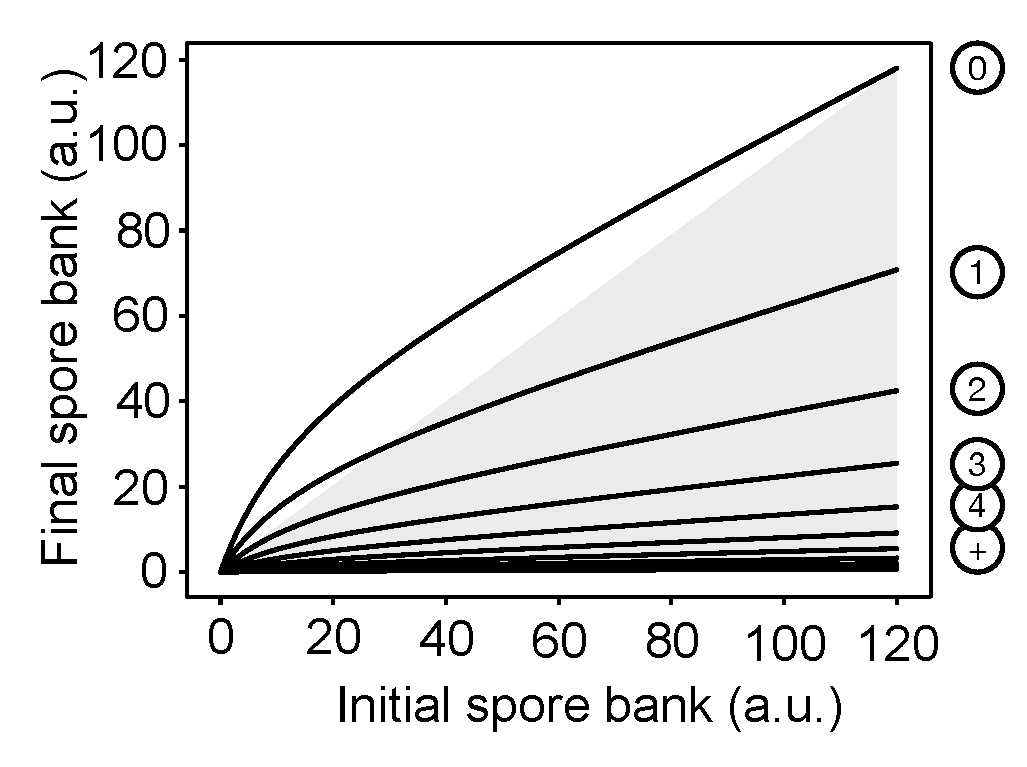
\includegraphics[width=0.75\columnwidth]{SCL_Fig/SCL_FigB.pdf}
\caption{\label{fig:figB}\textbf{Effect of break crops in the control of soil sclerotia after one season of oilseed rape.} The graph shows the spore bank value after one season of oilseed rape and 0 to 8 seasons of break crops, given a range of initial values of spore bank (0 to 100, in units of 1). In the shadowed area (grey), the final spore bank value is equal (diagonal) or lower than the initial spore bank value. }
\end{figure}
 
  \subsection{Single fungicide (F) and single genetic (G) control strategies.} 
  
  \textbf{Single strategy: application of fungicides (F).} To study the application of fungicides, we simulate 20 seasons of consecutive OSR where we apply fungicide ($\mu > 0$) at the beginning of each season. The reduction of infection compared to the null strategy $\varnothing$ is caused by the reduction of all the initial inocula $i_0$. Because fungicides can have different efficiencies -- depending on the drug and the dose -- we study the range of $\mu$ in decimal values, from 0 to 1. To understand the effect, we focus on the value of spore bank and cumulative yield at the end the 20th season  (Fig. \ref{figC}). Results show a quick drop from $\mu = 0.6$ ($S = 80.58$) to $\mu = 0.9$ ($S = 3.91$), where there is no build-up of soil sclerotia. The spore bank drop is reflected in the yield gain. We have a yield higher than 80\% for fungicide efficiency $\mu \geq 0.8$. 
  %Results show a spore bank drop from $\mu = 0.7$ to $\mu = 0.9$, value in which the final soil sclerotia is smaller than the initial ($S(t=20) = $). The spore bank drop is reflected in the yield, which final value is $>80\%$ of the maximum for $\mu \geq 0.8$.
 
 \textbf{Single strategy: use of a genetic resistant cultivar (G).}  To study the effect of cultivating oilseed rape variants with resistance, we simulate 20 seasons of consecutive OSR diminishing the pathogen fitness for the crop ($w < 1$). This reduces the rate of infection, compared to the null strategy $\varnothing$. The maximum infected host density, at the end of the 20th season, is, in consequence, lower. Because only variants with partial resistance are known, we define $w = 1 - \rho$ and we explore the range of $\rho$ in decimal values, from 0 to 1. As done with the fungicides, we study the final values of spore bank and yield at the end of 20 seasons  (Fig. \ref{figC}). Results show a sigmoidal decay of spore bank along the range of values. For $\rho \geq 0.6$, the final spore bank is smaller than the initial ($S(t=20) = 3.00$). The yield values show a sigmoidal increase where the final value is $>80\%$ of the maximum for $\rho \geq 0.4$.
 
 \begin{figure}
 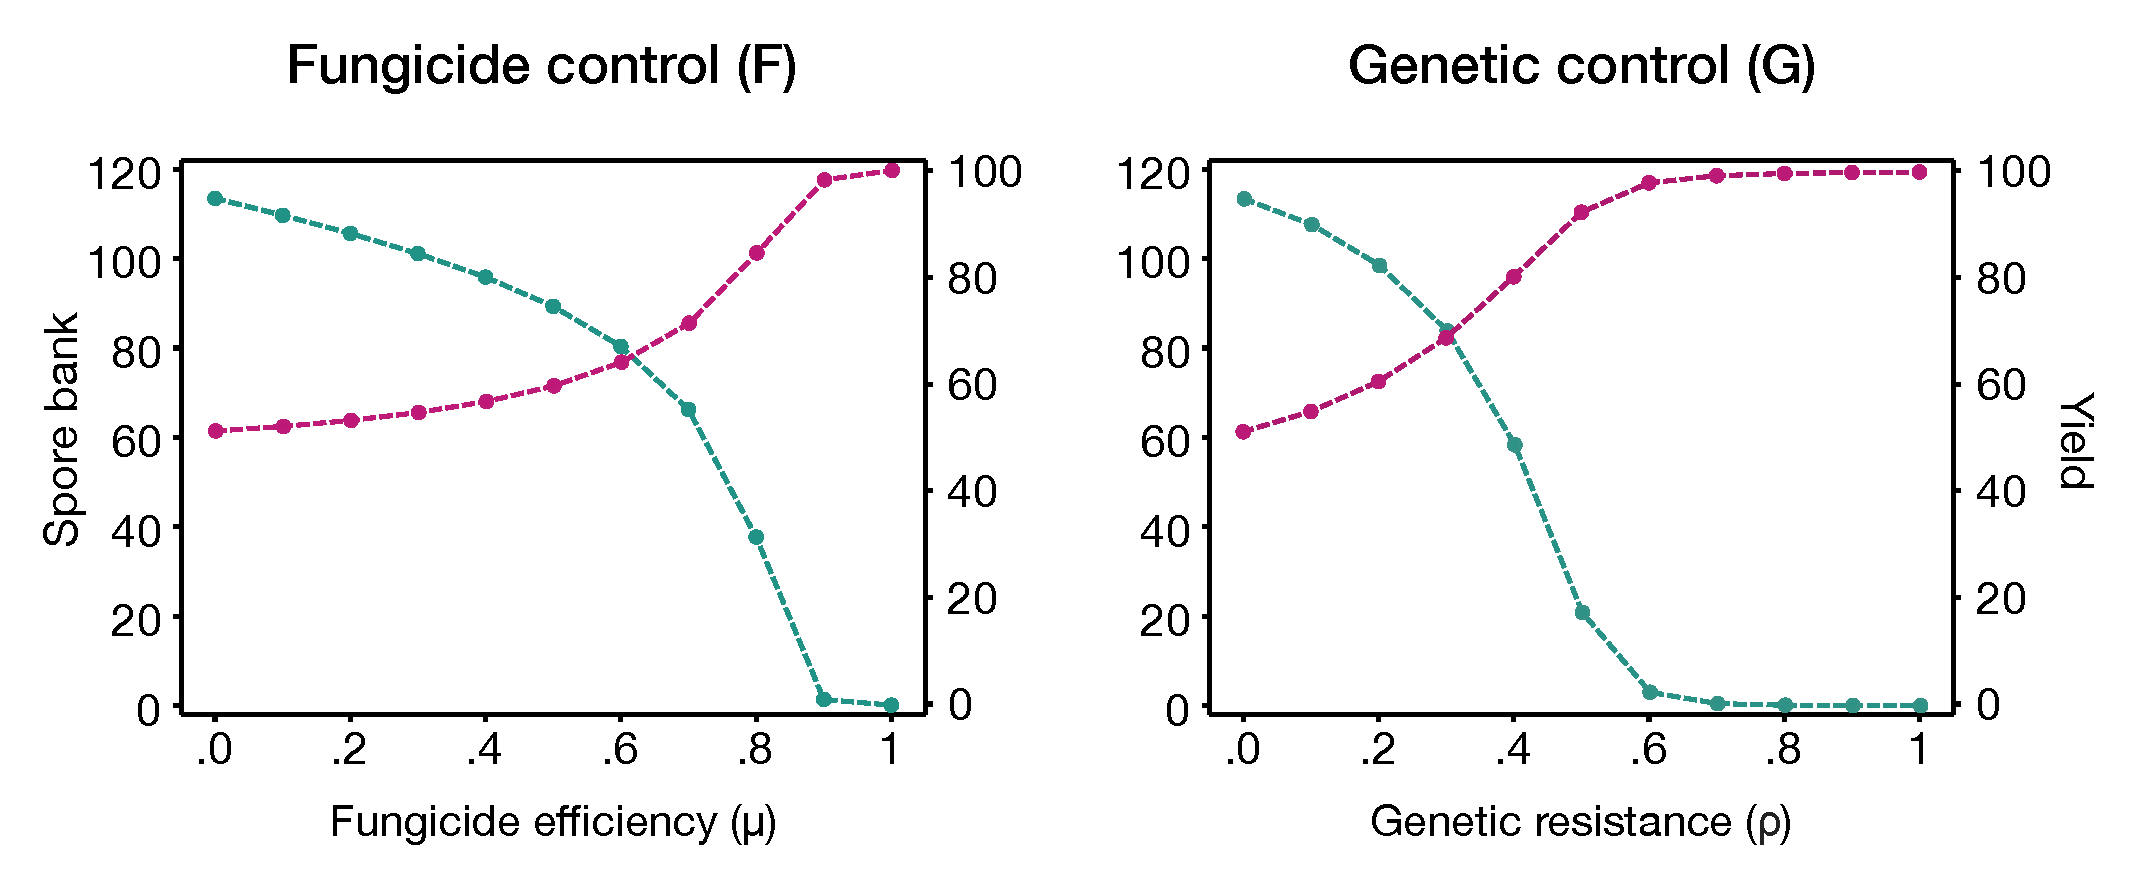
\includegraphics[width=\columnwidth]{SCL_Fig/SCL_FigC.pdf}
\caption{\label{fig:figC}\textbf{Spore bank and yield values after 20 seasons of fungicide (F) or genetic (G) control.} In the left panel, different values of fungicide efficiency $\mu$ are explored. In the right panel, different values of genetic resistance $\rho$ are explored. In both panels, we show the values of spore bank (blue) and yield (red) after 20 consecutive season of OSR with the corresponding control strategy. }
\end{figure}
 
\subsection{Integration of two control strategies: cultural-fungicide (CF), cultural-genetic (CG) and fungicide-genetic (FG) control} 

\textbf{Double control by cultural rotations and fungicides (CF)}. We combine rotations of OSR-BC (1 break crop season) with the application of fungicides in the OSR seasons  (Fig. \ref{figD}). We apply the same analysis than in the single fungicide control (F), simulating 20 seasons with alternations of OSR and BC. Results show that the final spore bank is generally reduced to less than half the values obtained with the single strategy. The final spore bank is smaller than the initial for $\mu \geq 0.8$. Yield is $>80\%$ of the maximum for $\mu \geq 0.6$, if we consider the maximum yield of reference the corresponding to OSR-BC alternations without infection. 
 
 \textbf{Double control by cultural rotations and genetic resistance (CG)}. We use rotations of OSR-BC (1 break crop season) by cultivating a variant with genetic resistance in the OSR seasons (Fig. \ref{figD}). We apply the same analysis than in the single genetic control (G), simulating 20 seasons with alternations of OSR and BC. The sigmoidal decay is maintained, with the values reduced to less than half the values of the single strategy. The final spore bank is smaller than the initial for $\rho \geq 0.4$. Yield is $>80\%$ of the maximum for $\mu \geq 0.3$, if we consider the maximum yield of reference the corresponding to OSR-BC alternations without infection. 

\textbf{Double control by fungicides and genetic resistance (GF)}. To compare the different fungicide efficiencies $\mu$ with different levels of genetic resistance $\rho$, we do a pairwise comparison and analyse for which values the final spore bank is smaller than the initial one (no build-up of the soil sclerotia) and for which values the final yield is $>80\%$ of the maximum (when consecutive OSR are cultivated without infection) (Fig. \ref{figE}). Results show that in 70.25\% of the combinations, there is no build-up of soil sclerotia; and in 80.17\% of the combinations, the yield is $>80\%$ of the maximum. For both, the space is more constrained by the level of fungicide efficiency than by the level of genetic resistance. 

\begin{figure}
 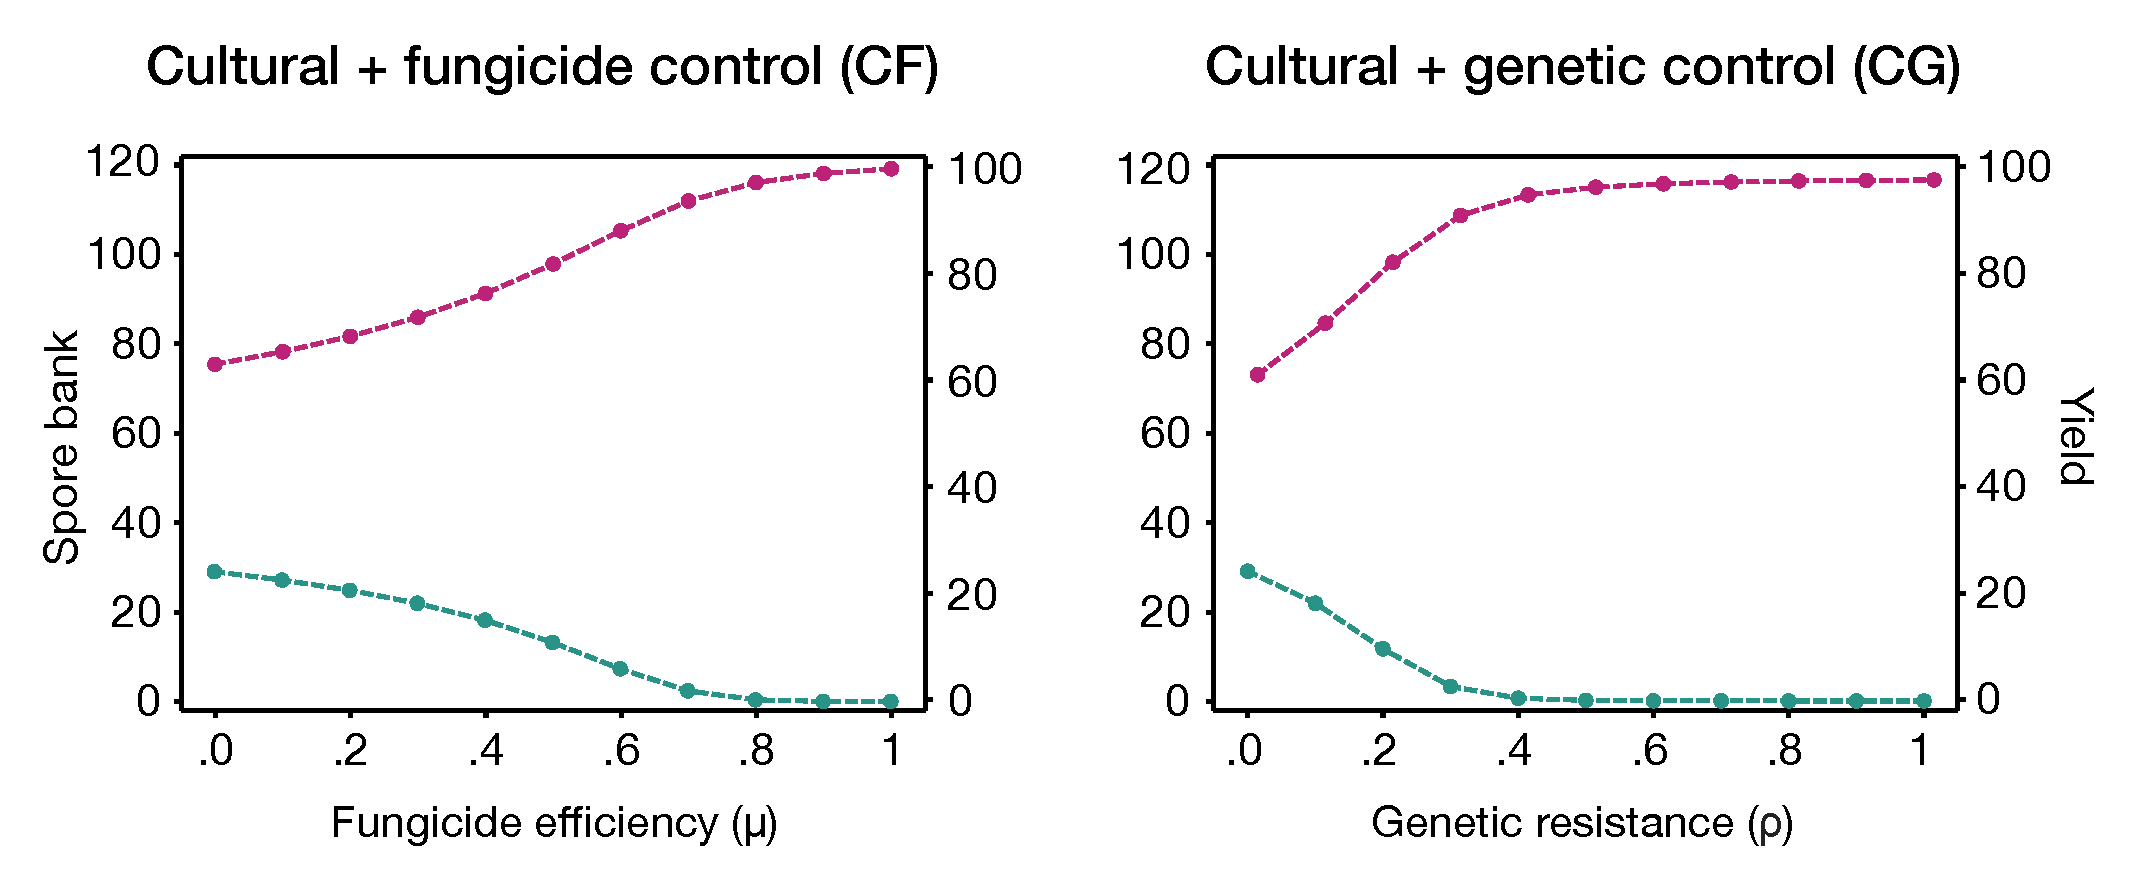
\includegraphics[width=\columnwidth]{SCL_Fig/SCL_FigD.pdf}
\caption{\label{fig:figD}\textbf{Spore bank and yield values after 20 seasons of cultural and fungicide (CF) or cultural and genetic (CG) control.} In the left panel, different values of fungicide efficiency $\mu$ are explored. In the right panel, different values of genetic resistance $\rho$ are explored. In both panels, we show the values of spore bank (blue) and yield (red) after 20 consecutive season of OSR with the corresponding control strategy. }
\end{figure}

 \begin{figure}
 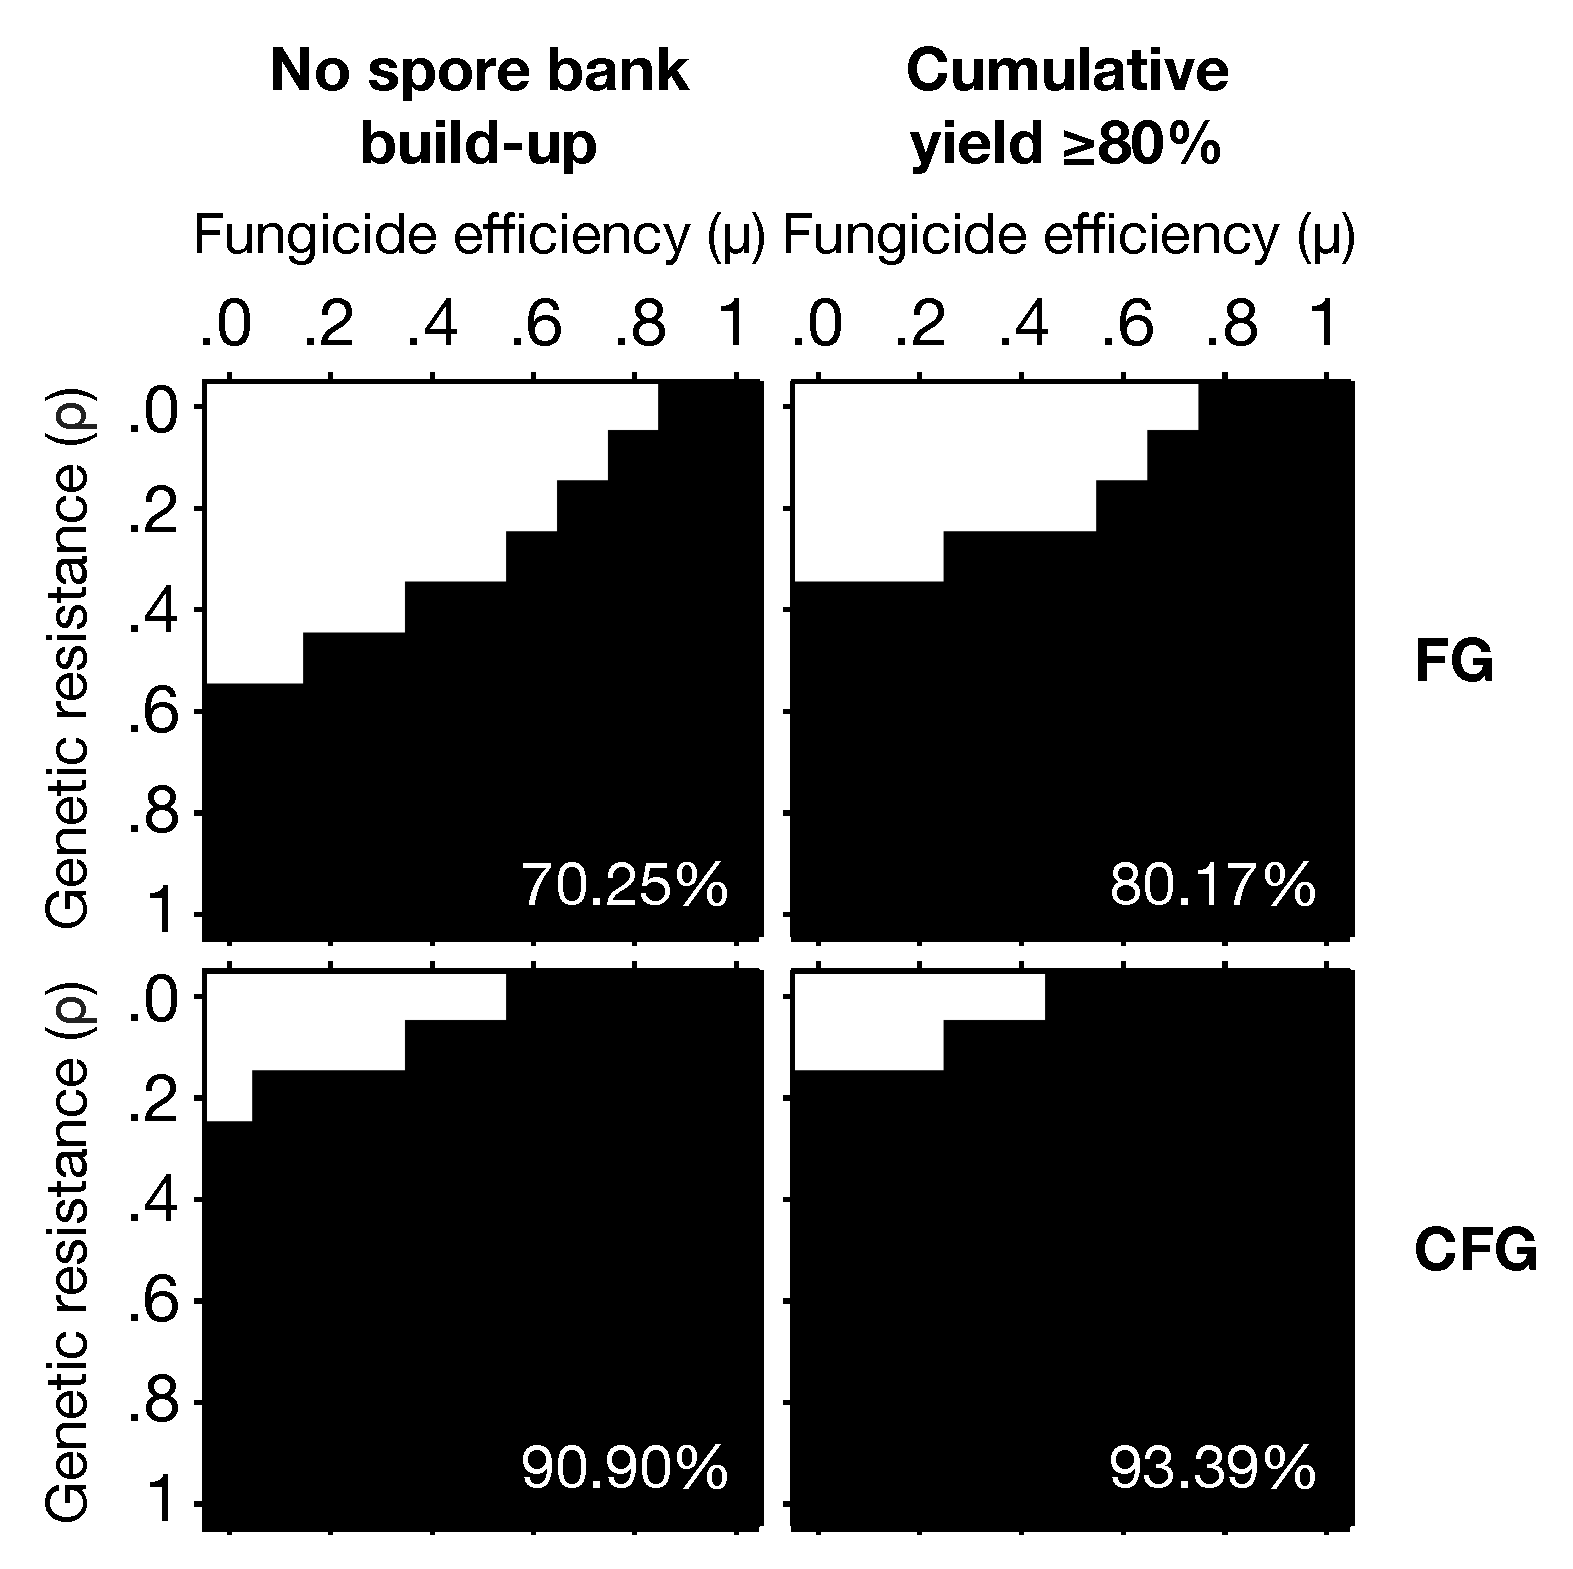
\includegraphics[width=\columnwidth]{SCL_Fig/SCL_FigE.pdf}
\caption{\label{fig:figE}\textbf{Final spore bank and final yield qualitative values for fungicide-genetic (FG) and cultural-fungicide-genetic (CFG) control strategy.} We calculate the final spore bank and the final yield after 20 seasons of combined fungicide-genetic control (FG) -- top pannel -- and combined cultural-fungicide-genetic control (CFG) -- bottom pannel --, for different values of genetic resistance ($\rho$, $y$ axis) and fungicide efficiency ($\mu$, $x$ axis). If the final spore bank is lower than the initial spore bank, there is no build-up (black); if it is higher, there is build-up (white). For the final yield, we set a threshold to 80\% of the maximum yield obtained with consecutive OSR cultivation (for FG) or with OSR-BC cultivation (for CFG), both without infection; and indicate if it yields equal or less (white) or more (black) than 80\%. The indicated percentages show the proportion of combinations of fungicide efficiency and resistance that allow infection control.}
\end{figure}

\subsection{Integration of three control strategies: cultural-fungicide-genetic (CFG) control}

The integration of three control strategies is modelled during 20 seasons in which (1) we use rotations of OSR-BC (1 break crop season), (2) we apply different values of fungicide efficiency $\mu$, and (3) we set different values of genetic resistance $\rho$ for the OSR crop. To study the effect of combining the three strategies, we do a pairwise comparison of values of $\mu$ and $\rho$ (as in the FG strategy) but for simulations in which OSR and BC have been alternated (instead of consecutive OSR)  (Fig. \ref{figE}).  Results show that in 90.90\% of the combinations, there is no build-up of soil sclerotia; and in 93.39\% of the combinations, the yield is $>80\%$ of the maximum when alternations of OSR-BC are cultivated without infection. Thus, the triple combination increases the space where infection control and maximisation of yield is possible. For both goals, the space is more constrained by the level of fungicide efficiency than by the level of genetic resistance. 


On the other hand, when we compare all eight strategies ($\varnothing$, C, F, G, CF, CG, FG, CFG) for high ($\mu = 0.8$) and low ($\mu = 0.2$) fungicide efficiency, and for high ($\rho = 0.8$) and low genetic resistance ($\rho = 0.2$), the triple control CFG performs best in both controlling the build-up (lowering the spore bank value to less than the initial value) and having a high yield (Fig. \ref{figF}).


 \begin{figure}
 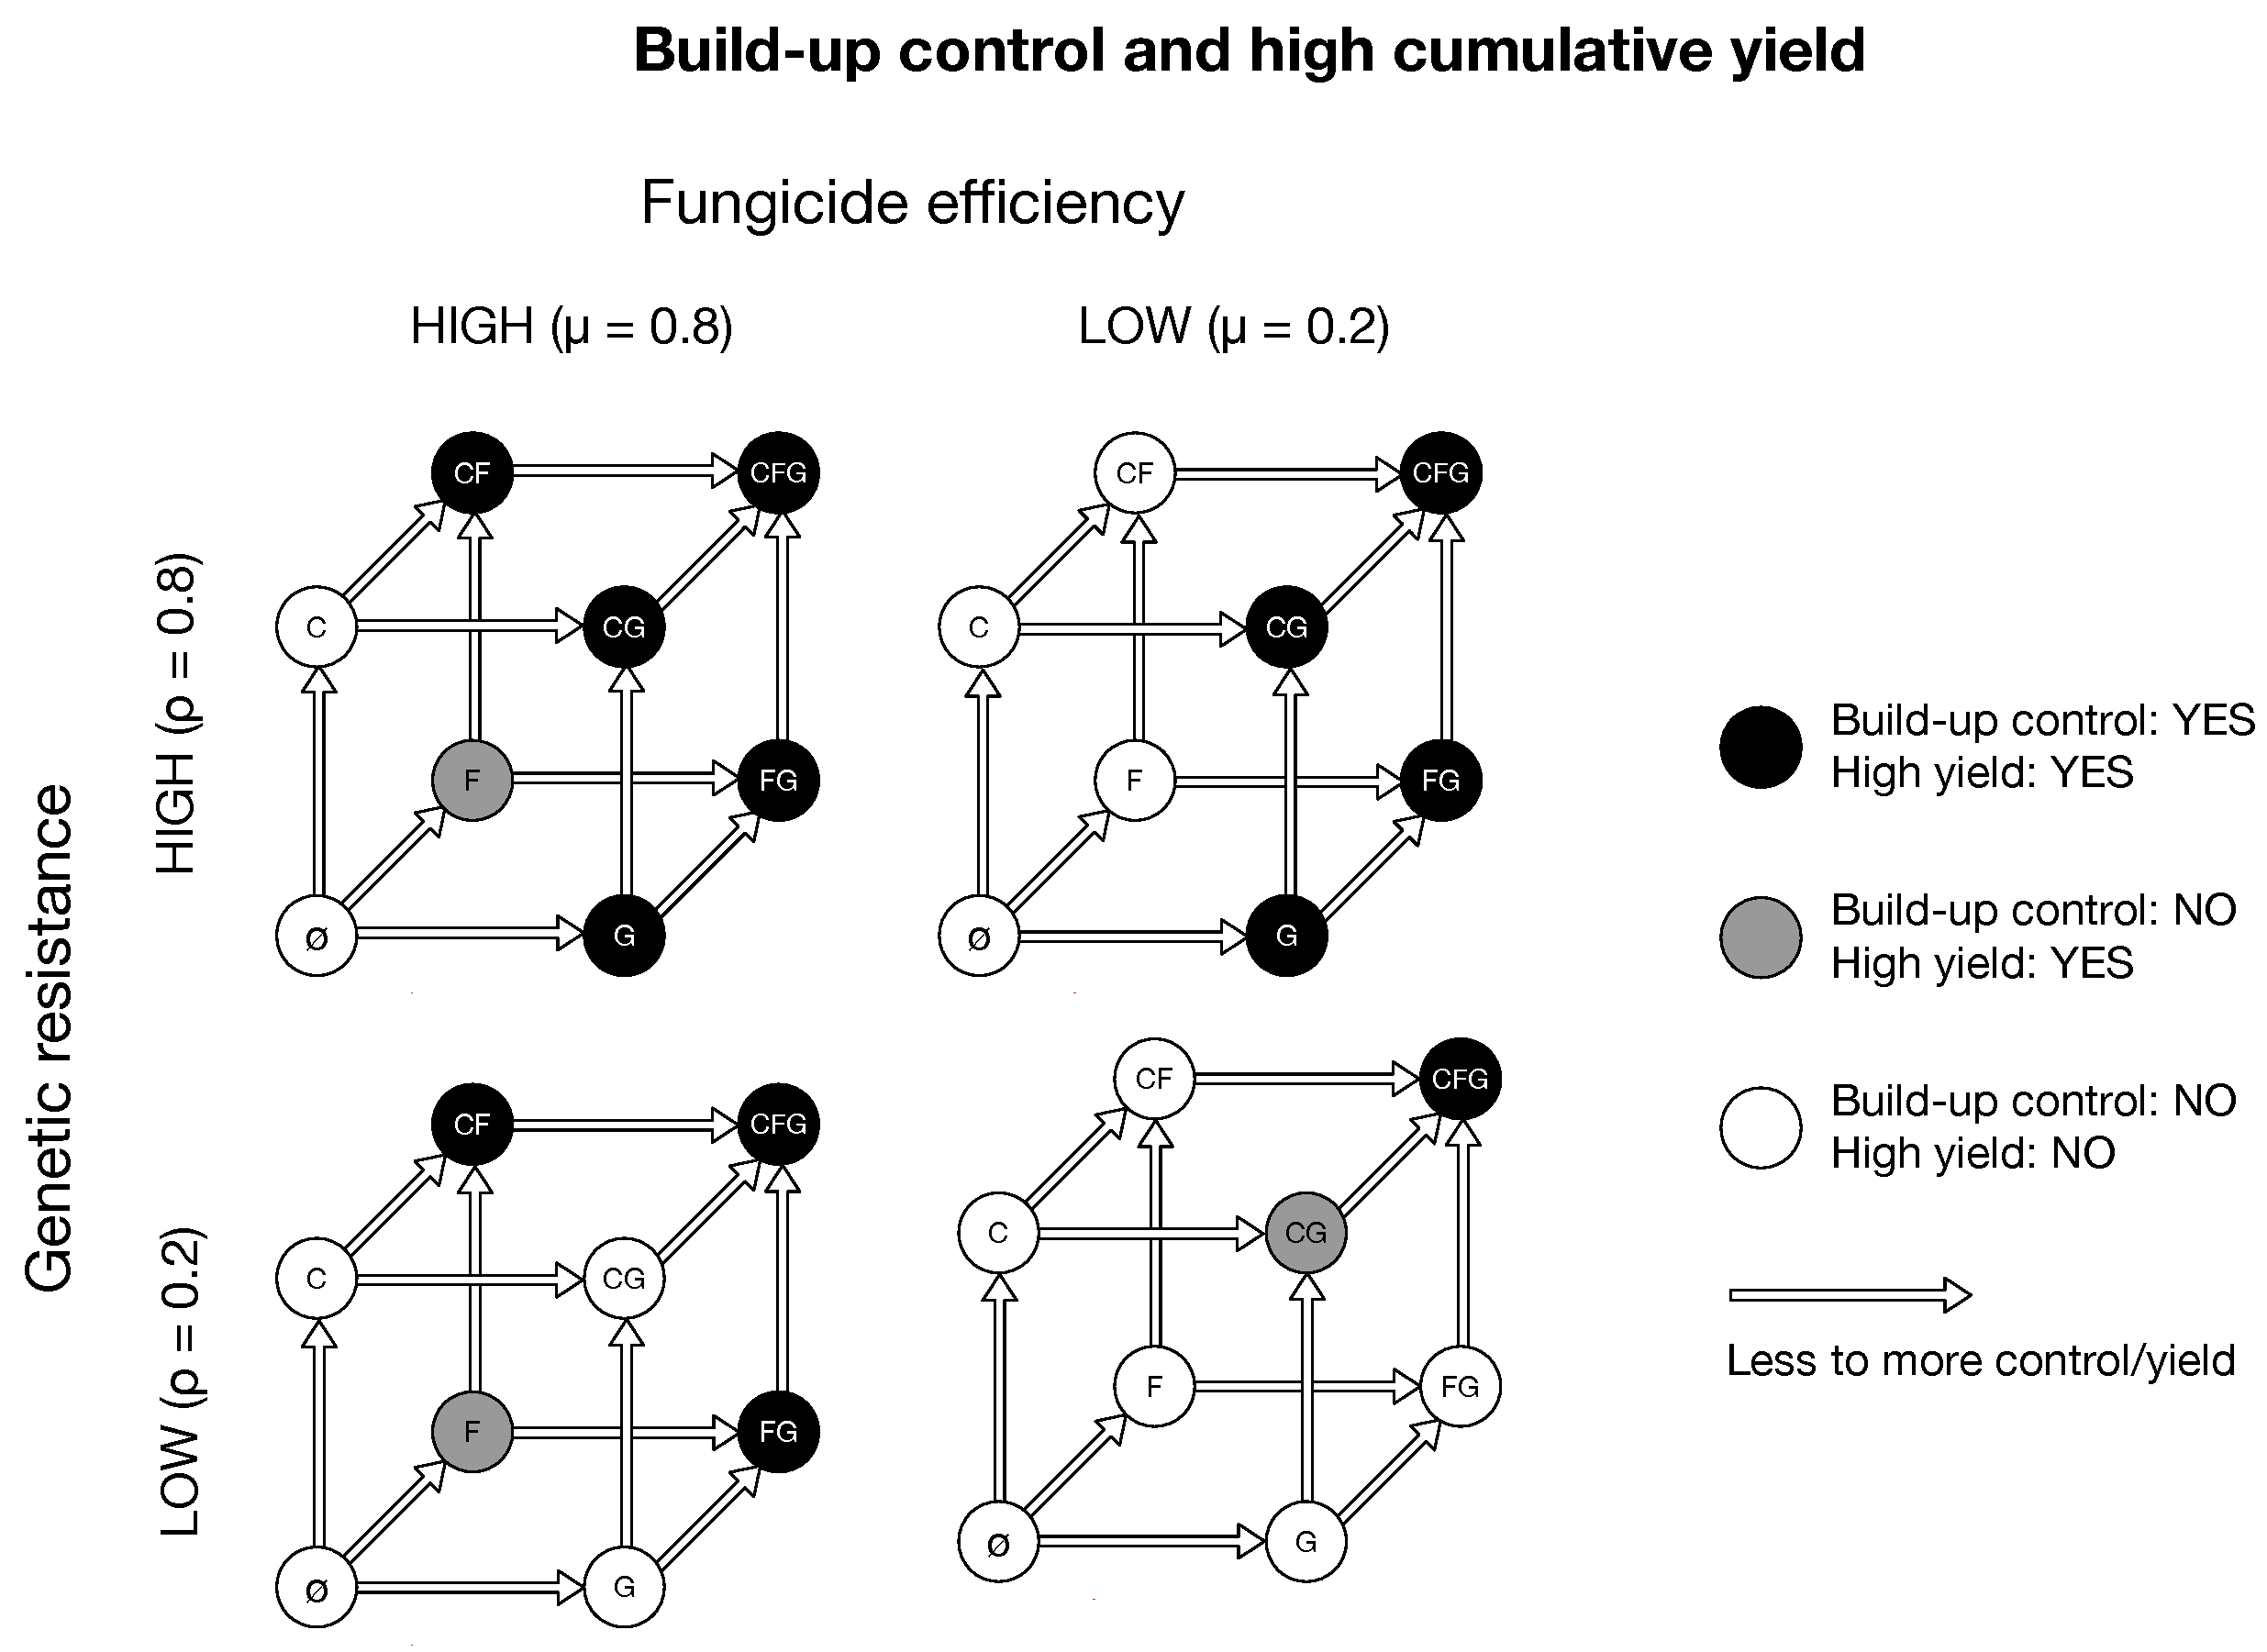
\includegraphics[width=\columnwidth]{SCL_Fig/SCL_FigF.pdf}
\caption{\label{fig:figF}\textbf{Comparison of all control strategies for build-up control and yield.}
We calculate the final spore bank and the final yield after 20 seasons for all strategies and compare if they control the build-up (i.e. the final spore bank is lower than the small one) and if they have high cumulative yield (i.e. the total yield after 20 seasons is higher than 80\% of the yield when grown without infection). We compare results when fungicide efficiency is high ($\mu = 0.8$) and low ($\mu = 0.2$), and for high genetic resistance ($\rho = 0.8$) and low genetic resistance ($\rho = 0.2$). Strategies do either (i) control the build up and yield high (black), (ii) not control the build up but yield high (grey), or (iii) not control the build-up and not yield high (white). In all cubes, arrows point to strategies that perform quantitatively better. }
\end{figure}

\section{Discussion}

 (to do)
 
 
\section{Next steps}

\textbf{Parameter optimisation using an algorithm.} Given a set of data which indicates field values for our model variables, we can find the parameter values that approximate the most our simulations to reality. As discussed in methods, we can relate the stem rot index (often indicated in field reports) with the percentage of infected host density, as both are indicators of percentage of crop damage. Other data indications such as number of apothecia could help estimating the spore bank in the field, and long term studies with consecutive seasons of OSR could help adjusting the build-up of the infection. An optimisation algorithm would test a range of parameter values for multiple parameters and indicate accurate values fitting the data. This would provide more reliability to our results. 

\textbf{Cost assessment of strategies}. In the model presented, we do not include any costs for the control strategies. For cultural control, the immediate cost is the reduction of cropping frequency of OSR; however break crops are cereals of commercial interest which can provide other benefits. On the other side, spraying fungicides is not always cost-effective: farmers are recommended to spray only if a yield loss higher than 25-30\% is expected, for the economic costs associated to the product and its application. Also, a cultivar with genetic resistance can carry yield penalties, associated to crop traits such as number of pods per plant or seeds per pod, which can vary due to resource reallocation. Including the costs can change the optimality of the strategies, as the economic costs of, for example the triple control CFG, could be higher than its benefits.


\textbf{Study of pathogen evolution.} As mentioned, we have assumed constant or durable effectivity of fungicide application or genetic resistance. However, this disregards pathogen evolution. \textit{Sclerotinia} resistance to fungicides is rare, due to its monocyclic life cycle. However, it has been reported in few cases, when fungicides were applied for 10 years or more. Pathogen virulence evolution for cultivars with partial resistance could evolve as well, lowering the effectivity of the genetic control.  





\bibliographystyle{naturemag}
\bibliography{\string~/Bibtex/et.bib}
%\bibliography{\string~/et-bib/et.bib}


\end{document}


